\section{Binning}
\label{sec:binning}
We achieve reproducible summation of floating point numbers through binning.
Each number is split into several components corresponding to predefined
exponent ranges, then the components corresponding to each range are
accumulated separately. We begin in Section \ref{sec:binning_bins} by
explaining the particular set of ranges (referred to as bins, see Figure~\ref{fig:binning}) used.
Section \ref{sec:binning_slices} develops mathematical theory to describe the
components (referred to as slices) corresponding to each bin.
The data format (called Indexed Type) to represent bins will be
explained in Section~\ref{sec:indexed}.
In this section, we develop 
theory to concisely describe and prove correctness of algorithms throughout the
paper (especially Algorithms \ref{alg:depositrestricted} and \ref{alg:deposit}).

\begin{figure}[H]
\begin{center}
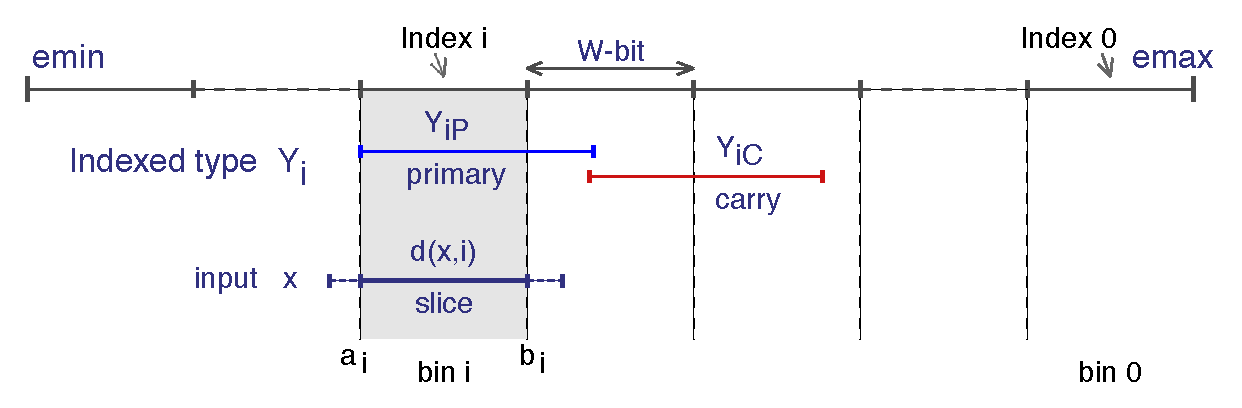
\includegraphics[width=\textwidth]{plots/indexedFP}
\caption{Indexed Floating-Point: binning process}
\label{fig:binning}
\end{center}
\end{figure}


    \subsection{Bins}
    \label{sec:binning_bins}
    We start by dividing the exponent range $(e_{\min} - p, ..., e_{\max} + 1]$
    into \textbf{bins} $(a_i, b_i]$ of \textbf{width} $W$ according to
    \eqref{eq:imax}, \eqref{eq:a}, and \eqref{eq:b}. Such a range is used so
    that the largest and smallest (denormalized) floating point numbers may be
    approximated.
    \begin{samepage}
    \begin{definition}
    \begin{align}
        i_{\max} & = \bigl\lfloor(e_{\max} - e_{\min} + p - 1)/W\bigr\rfloor - 1
            \label{eq:imax} \\
        a_i & = e_{\max} + 1 - (i + 1)W \text{ for } 0 \leq i \leq i_{\max}
            \label{eq:a} \\
        b_i & = a_i + W
            \label{eq:b}
    \end{align}
    \end{definition}
    \end{samepage}

    We say the bin $(a_{i_0}, b_{i_0}]$ is \textbf{greater} than the bin
    $(a_{i_1}, b_{i_1}]$ if $a_{i_0} > a_{i_1}$ (which is equivalent to both
    $b_{i_0} > b_{i_1}$ and $i_0 < i_1$).

    We say the bin $(a_{i_0}, b_{i_0}]$ is \textbf{less} than the bin
    $(a_{i_1}, b_{i_1}]$ if $a_{i_0} < a_{i_1}$ (which is equivalent to both
    $b_{i_0} < b_{i_1}$ and $i_0 > i_1$).

    We use $i \leq i_{\max} = \lfloor(e_{\max} - e_{\min} + p - 1)/W\rfloor - 1$
    to ensure that $a_i > e_{\min} - p + 1$ as discussed in Section
    \ref{sec:indexed_underflow_gradual}. This means that the greatest bin,
    $(a_{0}, b_{0}]$, is
    \begin{equation}
      (e_{\max} + 1 - W, e_{\max} + 1]
      \label{eq:binmax}
    \end{equation}

    and the least bin, $(a_{i_{\max}}, b_{i_{\max}}]$, is
    \begin{equation}
      \Bigl(e_{\min} - p + 2 + \bigl((e_{\max} - e_{\min} + p - 1)\mod W\bigr),
      e_{\min} - p + 2 + W + \bigl((e_{\max} - e_{\min} + p - 1)\mod W\bigr)\Bigr]
      \label{eq:binmin}
    \end{equation}

    Section \ref{sec:indexed_underflow_gradual} explains why the bottom of the exponent range
    \begin{equation*}
    \Bigl(e_{\min} - p, e_{\min} - p + 2 + \bigl((e_{\max} - e_{\min} + p - 1) \mod W\bigr)\Bigr]
    \end{equation*}
    is ignored.

    As discussed in \cite{repsum}, and explained again in Section~\ref{sec:primitiveops_renormalize},
    we must assume
    \begin{equation}
      W < p - 2
      \label{eq:wupper}
    \end{equation}

    As discussed in Section \ref{sec:indexed_overflow}, we must also assume
    \begin{equation}
      2 W > p + 1
      \label{eq:wlower}
    \end{equation}

    ReproBLAS uses both \texttt{float} and \texttt{double} floating point
    types. The chosen division of exponent ranges for both types is shown in
    Figure \ref{tbl:bins}. The rationale behind choices for $W$ and $K$ is explained in Section \ref{sec:primitiveops_restrictions}.

    \begin{table}[!htbp]
        \centering
        \begin{tabular}{ | l | l | l | p{5cm} |} \hline
            Floating-Point Type & \texttt{float} & \texttt{double}\\ \hline
            $e_{\max}$ & 127 & 1023\\ \hline
            $e_{\min}$ &  -126 & -1022 \\ \hline
            $p$ & 24 & 53 \\ \hline
            $e_{\min} - p$ & -140 & -1075 \\ \hline
            $W$ & 13 & 40 \\ \hline
            $i_{\max}$ & 19 & 51 \\ \hline
            $(a_0, b_0]$ & $(115, 128]$ & $(984, 1024]$\\ \hline
            $(a_{i_{\max}}, b_{i_{\max}}]$ & $(-132, -119]$ & $(-1056, -1016]$ \\ \hline
        \end{tabular}
        \caption{ReproBLAS Binning Scheme}
        \label{tbl:bins}
    \end{table}

    \subsection{Slices}
    \label{sec:binning_slices}
    Throughout the text we will refer to the \textbf{slice} of some $x \in \R$
    in the bin $(a_i, b_i]$ (see Figure~\ref{fig:binning}).
    $x$ can be split into several slices, each slice
    corresponding to a bin $(a_i, b_i]$ and expressible as the (possibly
    negated) sum of a subset of $\{2^e, e \in (a_i, b_i]\}$, such that the sum
    of the slices equals $x$ exacltly or provides a good approximation of $x$. Specifically, the slice
    of $x \in \R$ in the bin $(a_i, b_i]$ is defined recursively as $d(x, i)$
    in \eqref{eq:d}. We must define $d(x, i)$ recursively because it is not a
    simple bitwise extraction. The extraction is more complicated 
    because the splitting is performed using floating-point 
    instructions. There are many ways to implement the splitting 
    (using only integer instructions, only floating point instructions, 
    a mix of the two, or even special purpose hardware). This paper 
    focuses on using a majority of floating point instructions for portability and 
    for efficiency on architectures with different register
    sets for fixed and floating point operands.
    Floating point instructions also allow us to take advantage of the 
    rounding operations built in to floating point arithmetic.
    \begin{samepage}
    \begin{definition}
    \begin{equation}
    \begin{aligned}
      d(x,0) & = \roundtonearestinfty(x, a_0+1)\\
      d(x, i) & = \roundtonearestinfty\bigl(x - \sum\limits_{j=0}^{i - 1}d(x,j), a_i + 1\bigr)
        \text{ for } i > 0.
    \end{aligned}
      \label{eq:d}
    \end{equation}
    \end{definition}
    \end{samepage}

    We make three initial observations on the definition of $d(x, i)$. First,
    we note that $d(x, i)$ is well defined recursively on $i$ with base case
    $d(x, 0) = \roundtonearestinfty(x, a_0 + 1)$.

    Next, notice that $d(x, i) \in 2^{a_{i} + 1}\Z$.

    Finally, it is possible that $d(x, 0)$ may be too large to represent as a
    floating point number. For example, if $x$ is the largest finite floating point
    number, then $d(x,0)=\roundtonearestinfty(x, a_0+1)$ would be $2^{e_{max}+1}$.
    Overflow of this type is accounted for in Section \ref{sec:indexed_overflow}.
    Technical detail of how to handle this special case during the binning process
    will be explained in Section~\ref{sec:primitiveops_deposit}.

    Lemmas \ref{lem:dzero} and \ref{lem:dmiddle} follow from the definition of $d(x, i)$.

    \begin{samepage}
    \begin{lem}
      For all $i \in \{0, ..., i_{\max}\}$ and $x \in \R$ such that $|x| < 2^{a_i}$,
      $d(x, i) = 0.$
      \label{lem:dzero}
    \end{lem}
    \end{samepage}

    \begin{proof}
      We show the claim by induction on $i$.

      In the base case, $|x| < 2^{a_0}$, by \eqref{eq:round} we have
      $d(x, 0) = \roundtonearestinfty(x, a_0 + 1) = 0$.

      In the inductive step, we have $|x| < 2^{a_{i + 1}} < \ldots < 2^{a_0}$ by \eqref{eq:a}
      and by induction $d(x, i)= ... = d(x, 0) = 0$. Thus,
      \[
        d(x, i + 1) = \roundtonearestinfty\bigl(x - \sum\limits_{j = 0}^{i}d(x, j), a_{i + 1} + 1\bigr)
            = \roundtonearestinfty(x, a_{i+1} + 1)
      \]
      Again, since $x < 2^{a_{i+1}}$, by \eqref{eq:round} we have
      \(
        d(x, i + 1) = \roundtonearestinfty(x, a_{i + 1} + 1) = 0.
      \)
    \end{proof}

    \begin{samepage}
    \begin{lem}
      For all $i \in \{0, ..., i_{\max}\}$ and $x \in \R$ such that $|x| < 2^{b_i}$,
      $d(x, i) = \roundtonearestinfty(x, a_i + 1)$.
      \label{lem:dmiddle}
    \end{lem}
    \end{samepage}

    \begin{proof}
      The claim is a simple consequence of Lemma \ref{lem:dzero}.

      By  \eqref{eq:a} and \eqref{eq:b}, $|x| < 2^{b_i} = 2^{a_{i - 1}} < \ldots <2^{a_0}$.
      Therefore Lemma \ref{lem:dzero} implies $d(x, 0) = ... = d(x, i - 1) = 0$
      and we have
      \[
        d(x, i) = \roundtonearestinfty\bigl(x - \sum\limits_{j = 0}^{i - 1}d(x, j), a_{i} + 1\bigr)
            = \roundtonearestinfty(x, a_{i} + 1)
      \]
    \end{proof}

    Lemma \ref{lem:dzero}, Lemma \ref{lem:dmiddle}, and \eqref{eq:d} can be
    combined to yield an equivalent definition of $d(x, i)$ for all $i \in \{0,
    ..., i_{\max}\}$ and $x \in \R$.

    \begin{equation}
      d(x, i) = \begin{cases}
        0 \text{ if } |x| < 2^{a_i}\\
        \roundtonearestinfty(x, a_i + 1) \text{ if } 2^{a_i} \leq |x| < 2^{b_i}\\
        \roundtonearestinfty\bigl(x - \sum\limits_{j=0}^{i - 1}d(x,j), a_i + 1\bigr) \text{ if } 2^{b_i} \leq |x|
        \end{cases}
      \label{eq:d2}
    \end{equation}

    Theorem \ref{thm:dround} shows that sum of the slices of $x \in \R$
    provides a good approximation of $x$.

    \begin{samepage}
    \begin{thm}
      For all $i \in \{0, ..., i_{\max}\}$ and $x \in \R$,
      $|x - \sum \limits_{j = 0}^id(x, j)| \leq 2^{a_i}$.
      \label{thm:dround}
    \end{thm}
    \end{samepage}

    \begin{proof}
      We apply  \eqref{eq:round} and \eqref{eq:d2}
      \begin{align*}
        \bigl|x - \sum \limits_{j = 0}^{i}d(x, j)\bigr| & = \Bigl|\bigl(x - \sum \limits_{j = 0}^{i - 1}d(x, j)\bigr) - d(x, i)\Bigr| \\
         & = \Bigl|\bigl(x - \sum \limits_{j = 0}^{i - 1}d(x, j)\bigr) - \roundtonearestinfty\bigl(x - \sum \limits_{j = 0}^{i - 1}d(x, j), a_{i} + 1\bigr)\Bigr| \leq 2^{a_{i}}
      \end{align*}
    \end{proof}

    Although the bins do not extend all the way to $e_{\min} - p$, we now
    show that the sum of the slices of some $x \in \F$ still offers a good
    approximation of $x$.

    Using $W < p - 2$ and \eqref{eq:binmin},
    \begin{align*}
      a_{i_{\max}} & = e_{\min} - p + 2 + \bigl((e_{\max} - e_{\min} + p - 1 ) \mod W \bigr) \\
          & \leq e_{\min} - p + 2 + (W - 1) \\
          & < e_{\min} - p + 2 + (p - 2 - 1) =  e_{\min} - 1 
    \end{align*}

    Hence,
    \[
      a_{i_{\max}} \leq e_{\min} - 2
    \]

    As a consequence, we can use Theorem \ref{thm:dround} to say that for any $x \in \R$,
    \begin{equation}
      \bigl|x - \sum\limits_{i = 0}^{i_{\max}} d(x, i)\bigr| \leq 2^{a_{i_{\max}}} \leq 2^{e_{\min} - 2}
      \label{eq:droundunderflow}
    \end{equation}

    This means that we can approximate $x$ using the sum of its slices to the
    nearest multiple of $2^{e_{\min}-1}$.

    As the slices of $x$ provide a good approximation of $x$, the sum of the slices of some $x_0, ..., x_{n - 1} \in \R$ provide a good approximation of $\sum\limits_{j = 0}^{n - 1} x_j$. This is the main idea behind the reproducible summation algorithm presented here.
    Since the largest nonzero slices of $x$ provide the best approximation to $x$, we compute the sum of the slices of each $x_0, ..., x_{n - 1}$ corresponding to the largest $K$ bins such that at least one slice in the largest bin is nonzero. If such an approximation can be computed exactly, then it is necessarily reproducible.

    If the sums of slices corresponding to each bin are kept separate, we can compute the reproducible sum iteratively, only storing sums of nonzero slices in the $K$ largest bins seen so far. When a summand is encountered with nonzero slices in a larger bin that what has been seen previously, we abandon sums of slices in smaller bins to store the sums of slices in the larger ones.

    Before moving on to discussions of how to store and compute the slices and sums of slices, we must show a bound on their size. Theorem \ref{thm:dbound} shows a bound on $d(x, i)$.

    \begin{samepage}
    \begin{thm}
      For all $i \in \{0, ..., i_{\max}\}$ and $x \in \R$, $|d(x, i)| \leq 2^{b_i}$.
      \label{thm:dbound}
    \end{thm}
    \end{samepage}

    \begin{proof}
      First, we show that $|x - \sum\limits_{j=0}^{i - 1}d(x,j)| \leq 2^{b_i}$.

      If $i = 0$, then we have
      \begin{equation*}
        \bigl|x - \sum\limits_{j=0}^{i - 1}d(x,j)\bigr| = |x| < 2 \cdot 2^{e_{\max}} < 2^{b_0}
      \end{equation*}
      Otherwise, we can apply  \eqref{eq:a} and \eqref{eq:b} to Theorem \ref{thm:dround} to get
      \begin{equation*}
        \bigl|x - \sum \limits_{j = 0}^{i - 1}d(x, j)\bigr| \leq 2^{a_{i - 1}} = 2^{b_i}
      \end{equation*}

      As $2^{b_i} \in 2^{a_i + 1}\Z$,  \eqref{eq:d} can be used

      \begin{equation*}
        \bigl|d(x, i)\bigr| = \Bigl|\roundtonearestinfty\bigl(x - \sum\limits_{j=0}^{i - 1}d(x,j), a_i + 1\bigr)\Bigr| \leq 2^{b_i}
      \end{equation*}
    \end{proof}

  Combining Theorem \ref{thm:dbound} with the earlier observation that $d(x,i) \in 2^{a_i + 1}\Z$, we see that the slice $d(x, i)$ can be represented by bits lying in the bin $(a_i, b_i]$ as desired.

